\documentclass[aspectratio=169]{beamer}
\usetheme{SimplePlus}
\usecolortheme{default}

\usepackage{tikz}
\usepackage{amsmath}
\usepackage{amssymb}
\usepackage{isomath}
%\usepackage{bm}

\renewcommand{\vec}{\vectorsym}

\title[Finite Differences in 2D/3D \& Nonlinearities]{Finite Differences in 2D/3D and \\ Unavoidable Nonlinearities}
\author{Nicol\'as A. Barnafi}
\date{}

\begin{document}

\begin{frame}
    \titlepage
\end{frame}

\begin{frame}{Last class}
    $$\mathcal A u = f \qquad \text{discretize:}\qquad \mathbb A_h \vec u_h = \vec f_h $$
    \begin{block}{Lax Equivalence Theorem}
        If $\mathbb A_h$ is consistent of order $k$, then
        $$ \text{Convergence $O(h^k)$} \quad \Leftrightarrow \quad \text{Stability} $$
    \end{block}
\end{frame}

\begin{frame}{Outline}
    \tableofcontents
\end{frame}

\section{2D Domain Discretization}

\begin{frame}{Collocation and the discrete geometry}
    Extension to higher dimensions $\to$ tensor products.
    
    Set $\Omega = (a_x, b_x) \times (a_y, b_y)$ and an equispaced discrete grid $\Omega_h$:
    \begin{itemize}
        \item $a_x = x_0, \dots, x_{N_x-1} = b_x$
        \item $a_y = y_0, \dots, y_{N_y-1} = b_y$
    \end{itemize}
    \vspace{0.3cm}
    \begin{columns}
        \begin{column}{0.4\textwidth}
    Each grid point is given by:
    \[
        X_{i,j} := (x_i, y_j) 
    \]
    $\forall i,j \in \{0, \dots, N_x-1\} \times \{0, \dots, N_y-1\}$
        \end{column}
        \begin{column}{0.55\textwidth}

            \begin{center}
            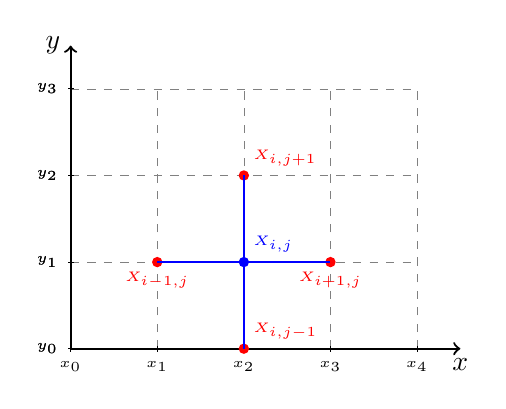
\begin{tikzpicture}[scale=1.1]
                % Grid
                \draw[step=1cm,gray,very thin, dashed] (0,0) grid (4,3);
                
                % Axes
                \draw[->, thick] (0,0) -- (4.5,0) node[anchor=north] {$x$};
                \draw[->, thick] (0,0) -- (0,3.5) node[anchor=east] {$y$};
                
                % Ticks
                \foreach \x in {0,1,2,3,4} \draw (\x, 1pt) -- (\x, -1pt) node[anchor=north] {\tiny $x_{\x}$};
                \foreach \y in {0,1,2,3} \draw (1pt, \y) -- (-1pt, \y) node[anchor=east] {\tiny $y_{\y}$};
                \foreach \y in {0,1,2,3} \draw (1pt, \y) -- (-1pt, \y) node[anchor=east] {\tiny $y_{\y}$};
                
                % Nodes & Stencil
                \fill[blue] (2,1) circle (0.06) node[anchor=south west] {\tiny $X_{i,j}$};
                \fill[red] (1,1) circle (0.06) node[anchor=north] {\tiny $X_{i-1,j}$};
                \fill[red] (3,1) circle (0.06) node[anchor=north] {\tiny $X_{i+1,j}$};
                \fill[red] (2,0.2) circle (0.00) node[anchor=west] {\tiny $X_{i,j-1}$};
                \fill[red] (2,2.2) circle (0.00) node[anchor=west] {\tiny $X_{i,j+1}$};

                \fill[red] (2,0) circle (0.06) node[anchor=west] {};
                \fill[red] (2,2) circle (0.06) node[anchor=west] {};
        
                % Connections
                \draw[thick, blue] (1,1) -- (3,1);
                \draw[thick, blue] (2,0) -- (2,2);
            \end{tikzpicture}
            \end{center}
        \end{column}
    \end{columns}

\end{frame}

\begin{frame}{Discrete functions}
    Given a discrete mesh: 
    \begin{block}{Matrix grid function}
    A matrix grid function of function $f: \Omega \to \mathbb{R}$ is
        $$f_{i,j} := f(X_{i,j}) \in \mathbb{R}^{N_x \times N_y}$$
    \end{block}

    \alert{Note that it is a \emph{matrix}}

\end{frame}

\begin{frame}{The Index Map: Flattening the Grid}
    To solve linear systems, we must flatten 2D matrices into 1D vectors.

    Define an index map $I: \{0, \dots, N_x-1\} \times \{0, \dots, N_y-1\} \to \{0, \dots, N_x N_y - 1\}$:
    \[
        I(i, j) = i + j N_x
    \]
    \pause This lexicographical map is invertible:
    \[
        I \mapsto (i(I), j(I)) := (I \bmod N_x, \lfloor I / N_x \rfloor)
    \]
    \pause Thus, we can uniquely define the 1D vector $\vec{f}_I$ representing the grid points:
    \[
        \vec f_I := f_{i(I), j(I)} = f(X_{i(I), j(I)}) \in \mathbb{R}^{N_x N_y}
    \]
\end{frame}

\begin{frame}{Discrete Differential Operators in 2D}
    Applying the standard centered difference scheme in each direction independently:
    \begin{align*}
        D_{xx} f(X_{i,j}) &= \frac{1}{h_x^2} \left( f_{i+1,j} - 2 f_{i,j} + f_{i-1,j} \right) = [A_h f(X_{i,j})]_{i,j} \\
        D_{yy} f(X_{i,j}) &= \frac{1}{h_y^2} \left( f_{i,j+1} - 2 f_{i,j} + f_{i,j-1} \right) = [f(X_{i,j}) A_h^\top]_{i,j}
    \end{align*}
    
    where $A_h$ is the standard 1D discrete second derivative matrix. 
    
    \pause
    \begin{example}
    For the Poisson problem $-\Delta u = f$, the matrix equation before vectorization is:
    \[
        -\Delta u(X_{i,j}) \approx A_h U_h + U_h A_h^\top = F
    \]
    \end{example}
\end{frame}

\section{Kronecker Products and Assembly}

\begin{frame}{The Kronecker Product}
    To formalize the transition to the 1D vector space, we introduce the Kronecker product $\otimes : \mathbb{R}^{m \times n} \times \mathbb{R}^{p \times q} \to \mathbb{R}^{mp \times nq}$:
    \[
    A \otimes B :=
    \begin{pmatrix}
        A_{11}B & A_{12}B & \dots & A_{1n}B \\
        A_{21}B & A_{22}B & \dots & A_{2n}B \\
        \vdots & \vdots & \ddots & \vdots \\
        A_{m1}B & A_{m2}B & \dots & A_{mn}B
    \end{pmatrix}
    \]
    This operation is critical to rigorously define the sparse operator matrix for higher dimensions.
\end{frame}

\begin{frame}{Example}
    \begin{example}
        For $I=\left(\begin{smallmatrix}1&0 \\ 0&1 \end{smallmatrix}\right)$, $A = \left(\begin{smallmatrix}1&2\\3&4\end{smallmatrix}\right)$:
        $$ I\otimes A = \begin{bmatrix} 1 A & 0 \\ 0 & 1 A \end{bmatrix} = \begin{bmatrix} 1 & 2 & 0 & 0 \\ 3 & 4 & 0 & 0 \\ 0 & 0 & 1 & 2 \\ 0 & 0 & 3 & 4
        \end{bmatrix} $$
    \end{example}

\end{frame}

\begin{frame}{Vectorization Lemma}
    \textbf{Lemma:} Let $A \in \mathbb{R}^{m \times n}$, $B \in \mathbb{R}^{p \times q}$ and $X \in \mathbb{R}^{q \times n}$. Denote the vector form of matrix $X$ as $X_I$. Then:
    \[
        (B \alert{X} A^\top)_I = (A \otimes B) \alert{X_I}
    \]
    
    \textit{Proof Sketch:} Expanding the right-hand side,
    \[
    (A \otimes B) X_I = 
    \begin{pmatrix}
        \sum_i A_{1i} B X_i \\
        \vdots \\
        \sum_i A_{mi} B X_i
    \end{pmatrix}
    =
    \begin{pmatrix}
        B X A_1^\top \\
        \vdots \\
        B X A_m^\top
    \end{pmatrix}
    = (B X A^\top)_I
    \]
    where $A_i$ are the rows of $A$, and $X_i$ are the columns of $X$.
\end{frame}

\begin{frame}{Assembling the 2D Discrete Laplacian}
    We had
    $$ A_h U_h + U_h A_h^\top = F_h $$
    and the Vectorization Lemma: $(BXA^T)_I = (A\otimes B)X_I$ yield:
    \begin{align*}
        (A_h U_h + U_h A_h^\top)_I &= (F_h)_I \\ 
        (A_h U_h I_h + I_h U_h A_h^\top)_I &= (F_h)_I \\ 
        (I_h \otimes A_h) u_I + (A_h\otimes I_h) u_I &= f_I
    \end{align*}

    Finally we get the matrix representation: 
    \[
        D_h^2 = A_h \otimes I + I \otimes A_h
    \]
    This rigorous construction naturally produces the block-tridiagonal sparsity pattern.
\end{frame}

\section{Extension to 3D}

\begin{frame}{3D Finite Differences: Geometry}
    This systematic approach extends to 3D domains $\Omega = (a_x, b_x) \times (a_y, b_y) \times (a_z, b_z)$. The index map becomes:
    \[
        I(i,j,k) = i + j N_x + k N_x N_y
    \]
    \begin{center}
    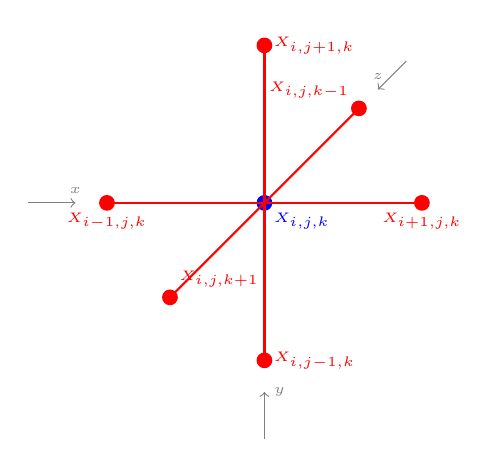
\begin{tikzpicture}[scale=2, z=-0.6cm]
        % Axes hints
        \draw[->, gray, thin] (-1.5,0,0) -- (-1.2,0,0) node[anchor=south] {\tiny $x$};
        \draw[->, gray, thin] (0,-1.5,0) -- (0,-1.2,0) node[anchor=west] {\tiny $y$};
        \draw[->, gray, thin] (0,0,-1.5) -- (0,0,-1.2) node[anchor=south] {\tiny $z$};

        % Central node
        \fill[blue] (0,0,0) circle (0.05) node[anchor=north west] {\tiny $X_{i,j,k}$};
        
        % X axis
        \draw[thick, red] (-1,0,0) -- (1,0,0);
        \fill[red] (-1,0,0) circle (0.05) node[anchor=north] {\tiny $X_{i-1,j,k}$};
        \fill[red] (1,0,0) circle (0.05) node[anchor=north] {\tiny $X_{i+1,j,k}$};
        
        % Y axis
        \draw[thick, red] (0,-1,0) -- (0,1,0);
        \fill[red] (0,-1,0) circle (0.05) node[anchor=west] {\tiny $X_{i,j-1,k}$};
        \fill[red] (0,1,0) circle (0.05) node[anchor=west] {\tiny $X_{i,j+1,k}$};
        
        % Z axis
        \draw[thick, red] (0,0,-1) -- (0,0,1);
        \fill[red] (0,0,-1) circle (0.05) node[anchor=south east] {\tiny $X_{i,j,k-1}$};
        \fill[red] (0,0,1) circle (0.05) node[anchor=south west] {\tiny $X_{i,j,k+1}$};
    \end{tikzpicture}
    \end{center}


\end{frame}

\begin{frame}{The 3D 7-Point Stencil}
    The discrete Laplacian $D_h^2$ operator is built via multiple Kronecker products:
    \[
        D_h^2 = A_h \otimes I \otimes I + I \otimes A_h \otimes I + I \otimes I \otimes A_h
    \]
    For a uniform grid $h = \Delta x = \Delta y = \Delta z$, this results in the standard \textbf{7-point stencil}.

\end{frame}

\section{Unavoidable Nonlinearities}

\begin{frame}{Unavoidable Nonlinearities}
    Often, stationary PDEs inherently possess nonlinearities. Consider a simple 1D boundary value problem:
    \begin{align*}
        -u'' + \sin(u) &= 0 \quad \text{in } (a, b) \\
        u(a) &= u_a, \quad u(b) = u_b
    \end{align*}
    
    Discretizing on a grid yields the nonlinear algebraic system:
    \[
        -\frac{1}{h^2}(u_{i+1} - 2u_i + u_{i-1}) + \sin(u_i) = 0
    \]
    with $u_0 = u_a$ and $u_N=u_b$. This is a root-finding problem $\mathcal{F}(u_h) = 0$, defined compactly as:
    \[
        \mathcal{F}(u_h) := A_h u_h + \sin(u_h) = 0
    \]
\end{frame}

\begin{frame}{Newton-Raphson: Linearization}
    To solve $\mathcal{F}(x) = 0$, Newton's method uses a Taylor expansion to linearize around a known iteration $x_k$:
    \[
        \mathcal{F}(x_{k+1}) \approx \mathcal{F}(x_k) + \nabla \mathcal{F}(x_k) \cdot \delta x_{k+1} = 0
    \]
    where $\delta x_{k+1} = x_{k+1} - x_k$. For our problem, the $i$-th component of $\mathcal{F}$ is:
    \[
        [\mathcal{F}(u_h)]_i = -\frac{1}{h^2}(u_{i-1} - 2u_i + u_{i+1}) + \sin(u_i)
    \]
    Differentiating with respect to $u_j$ gives the Jacobian entries:
    \[
        [\nabla \mathcal{F}(u_h)]_{i,j} = \frac{\partial [\mathcal{F}(u_h)]_i}{\partial u_j} = 
        \begin{cases}
            -1/h^2 & j \in \{i-1, i+1\} \\
            2/h^2 + \cos(u_i) & j = i \\
            0 & \text{elsewhere}
        \end{cases}
    \]
\end{frame}

\begin{frame}{Newton-Raphson: The Scheme}
    We can write the Jacobian compactly as:
    \[
        \nabla \mathcal{F}(u_h) = A_h + \text{diag}(\cos(u_h))
    \]
    The resulting \textbf{tangent system} to solve at each step $k$ is:
    \[
        \left[ A_h + \text{diag}(\cos(u_h^k)) \right] \delta u_h^{k+1} = - \left[ A_h u_h^k + \sin(u_h^k) \right]
    \]
    Followed by the update:
    \[
        u_h^{k+1} = u_h^k + \delta u_h^{k+1}
    \]
    \vspace{0.3cm}
    \textbf{Note:} Newton-Raphson is fast (quadratic conv.), but theory only guarantees \textbf{local convergence}.
\end{frame}

\begin{frame}{Picard Iteration (Fixed Point)}
    Alternative: "delay" the evaluation of the nonlinearity.     
    \[
        -\Delta u^{k+1} + \sin(u^k) = 0
    \]
    At the discrete level, this yields the fixed-point iteration:
    \[
        A_h u_h^{k+1} = - \sin(u_h^k)
    \]
    
    At converges it yields previous $u$... But does it converge?
\end{frame}

\begin{frame}{Convergence Proof of the Picard Scheme}
    Subtracting two consecutive Picard iterations gives the \textbf{error equation}:
    \[
        A_h (u_h^{k+1} - u_h^k) = -(\sin(u_h^k) - \sin(u_h^{k-1}))
    \]
    Recall that $A_h$ satisfies a discrete stability estimate $\|v_h\|_{\infty,h} \le C \|A_h v_h\|_{\infty,h}$. Applying this to our error equation:
    \begin{align*}
        \|u_h^{k+1} - u_h^k\|_{\infty,h} &\le C \|A_h(u_h^{k+1} - u_h^k)\|_{\infty,h} \quad \text{(Stability)} \\
        &= C \|-(\sin(u_h^k) - \sin(u_h^{k-1}))\|_{\infty,h} \quad \text{(Error equation)} \\
        &\le C \|u_h^k - u_h^{k-1}\|_{\infty,h} \quad \text{($\sin$ is 1-Lipschitz)}
    \end{align*}
    By the Banach fixed point theorem, if $C < 1$, the map is a contraction, and the Picard scheme is theoretically guaranteed to converge.
\end{frame}

\begin{frame}{Note on ordering}
    Should we discretize the algorithm or the equation?
\end{frame}

\begin{frame}{Summary}
    \begin{itemize}
        \item \textbf{Higher Dimensions:} Index remapping for flattening objects
        \item \textbf{Matrix Assembly:} Vectorization Lemma
        \item \textbf{Nonlinearities:} 
            \begin{itemize}
                \item Newton-Raphson (fast [quadratic] but local, requires Jacobian assembly) 
                \item Picard Iteration (slower [linear], fixed operator, convergent if contraction).
            \end{itemize}
    \end{itemize}
    \vspace{0.5cm}
\end{frame}

\begin{frame}
    \maketitle
\end{frame}
\end{document}
